%preamble - package inclusion and set up
\input{setup/preamble.tex}

%macros - please read this file
\input{setup/macros.tex}

\begin{document}       % TIP: If you are using TeXstudio you can open
%\tableofcontents      %      the file by Ctrl+LeftClick on setup/macros.tex
%\pagebreak             %      If the file doesn't exist, you will be asked
					   %      weather or not you want to create it.
%\begin{center}
%	\vspace{5cm}
%	\Huge{Worksheets}
%\end{center}
%\clearpage

%||||||||||||||||||||||||||||||||||||||||||||||||||||||||||||||||
%|||||||                 Example Inputs                  ||||||||
%||||||||||||||||||||||||||||||||||||||||||||||||||||||||||||||||
%|||||||                                                 ||||||||
%			 \input{chapters/aFigureSample.tex}			 %|||||||
%			 \input{chapters/bTableSample.tex} 		     %|||||||
%			 \input{chapters/cEquationSample.tex}		 %|||||||
%			 \input{chapters/dTikzSample.tex}            %|||||||
%			 \input{chapters/eCodeSample.tex}            %|||||||
%|||||||                                                 ||||||||
%||||||||||||||||||||||||||||||||||||||||||||||||||||||||||||||||
%||||||||||||||||||||||||||||||||||||||||||||||||||||||||||||||||


%%% Prereport %%%
		\setlength\cftaftertoctitleskip{2pt}
		\setlength\cftafterloftitleskip{6pt}
		\setlength\cftafterlottitleskip{6pt}
%\selectlanguage{danish}

%%% Frontmatter Settings %%%
		\pagestyle{empty} %disable headers and footers
		\pagenumbering{roman} %use roman page numbering in the frontmatter I II...
	%	\fancyfoot[RE,LO]{18??} %page number on all pages
		\fancyfoot[LE,RO]{\thepage}
		\fancyhead[LE,LO,RE,RO]{}

%%% Introductory Formalities %%%
%\includepdf[pages={1}]{formalities/frontpage.tex}
			\clearpage
\thispagestyle{empty}

\begin{figure}[H]
	\raggedleft
	\includegraphics[width=0.2\textwidth]{figures/aaulogo-en.png}
\end{figure} 

\vspace{5 cm}

\begin{center}
	\begin{Huge}
		\textbf{Evaluation of Electrotactile Feedback Schemes in a
			Closed-Loop Myoelectric Prosthesis}\\
		\vspace{5 mm}
		Master Thesis \\
		Biomedical Engineering \& Informatics \\ Spring $2019$\\
		\vspace{3 mm}
	\end{Huge}
	{\Large Project group: $19$gr$10407$} \\
	\vspace{1cm}
	\large{Christian Korfitz Mortensen, Martin Alexander Garenfeld}
\end{center}
\vspace*{\fill}

\begin{center}
	\line(1,0){400}
\end{center}

%\newpage
%
%\large{\textbf{Project period:}\\
%P7, Autumn 2017\\
%01/08/2017 - 20/12/2017\\
%
%\textbf{Project group:}\\
%17gr7404\\} %\fxnote{Input group number}
%
%
%\begin{center}
%	\Large{\textbf{Collaborators:}\\
%		\vspace{1.5cm}
%	\rule{10cm}{1pt}\\
%	Irene Uriarte \\
%	
%	\rule{10cm}{1pt}\\
%	Martin Alexander Garenfeld \\
%	
%	\rule{10cm}{1pt}\\
%	Oliver Thomsen Damsgaard \\
%	
%	\rule{10cm}{1pt}\\
%	Simon Bruun \\}
%\end{center}
%
%
%
%\large{\textbf{Supervisors:}\\
%Strahinja Dosen \\
%Jakob Lund Dideriksen \\
%Lotte N.S. Andreasen Struijk} \\
%\\
\newpage
			% <--- the frontpage
			\pagestyle{fancy}
%\include{formalities/kolofon}
			%\begin{document} 
\thispagestyle{empty}
\begin{titlepage}
	\begin{nopagebreak}
		{\samepage 
			
			\begin{tabular}{r}
				\parbox{\textwidth}{  \raisebox{-15mm}{\includegraphics[height=3cm]{figures/aaulogo-en.png}}
					\hfill \hspace{2cm} \parbox{8cm}{\begin{tabular}{l} %4.90
							{\small \textbf{\textcolor{aaublue}{Master Thesis}}}\\
							{\small \textbf{\textcolor{aaublue}{School of Medicine and Health}}}\\
							%{\small \textbf{\textcolor{aaublue}{Communication Technologies}}}\\ 
							{\small \textbf{\textcolor{aaublue}{Biomedical Engineering and Informatics}}}\\
							{\small \textcolor{aaublue}{Fredrik Bajers Vej 7A}} \\
							{\small \textcolor{aaublue}{9220 Aalborg}} \\
							%{\small \textcolor{aaublue}{\emph{http://www.sict.aau.dk/electronics-and-it}}}
				\end{tabular}}}
			\end{tabular}
			
			\begin{tabular}{cc}
				\parbox{7cm}{
					
					\textbf{Title:}
					
					Evaluation of Electrotactile Feedback Schemes in a
					Closed-Loop Myoelectric Prosthesis \\ 
					
%					\textbf{Theme:}
%					
%					\small{
%						Applied Biomedical Engineering and Informatics\\
%					}
					
					
					\parbox{8cm}{
						
						
						\textbf{Project period:}\\
						01/02/2019 - 6/6/2019\\
						
						\textbf{Project group:}\\
						10gr10407\\ %\fxnote{Input group number}
						
						\textbf{Participants:}\\
						Christian Korfitz Mortensen\\
						Martin Alexander Garenfeld\\
						
						
						
						\textbf{Supervisors:}\\
						Strahinja Dosen\\
						Jakob Lund Dideriksen\\
						
						
					}\\
					\\
					\\
					\textbf{Paper:} 10 pages \\
					\textbf{Worksheets:} 39 pages \\ 
					\textbf{Appendix:} 10 pages \\
					%\textbf{Ekstra:} For projektkode: Se forord\\ %eks. en CD eller USB
					\textbf{Concluded:} 6/6/2019\\
					\\
					\textit{The content of this report is freely available, but publication (with reference) may only be done with
						agreement with the authors.}
					\vfill } &
				\parbox{7cm}{
					\vspace{-.55cm}
					\hfill
					\vspace{.55cm}
					\begin{tabular}{l}
						{\textbf{Abstract:}} \\
						\fbox{
							\parbox{8.5cm}{\bigskip
								{\vfill{\small {\small text
\vspace{-0.5cm}}
										\bigskip}}
						}}
				\end{tabular}}
		\end{tabular}} %\vspace{1cm}
		
		
		%\centering
		%\textit{Offentliggørelse af rapportens indhold, med kildeangivelse, må kun ske efter aftale med forfatterne.}\\
		
	\end{nopagebreak}
\end{titlepage}
%\end{document} 			 % <--- the titlesheet - contains the synopsis!!
%%% Preface %%%
			\cleardoublepage
			
%			{\small text
\vspace{-0.5cm}}			 % <--- this is the abstract!!
\clearpage
			\input{formalities/forord.tex}				% <--- the preface
%
%\input{contents/bBackground/title.tex}
\clearpage
			\pdfbookmark[0]{Table of Contents}{label: tableOfCentents}
			\tableofcontents
			\cleardoublepage


%%% Mainmatter Settings %%%
\pagenumbering{arabic} %use arabic page numbering in the mainmatter
\fancyhf{}
\fancyfoot[C]{\thepage} %\text{ of} \pageref{LastPage}			% ADD LABLE{LASTPAGE} TO LAST PAGE !!
\fancyfoot[RE,LO]{19gr10407}																								   %
\fancyhead[RE,LO]{}																												%% } consider fancyfoots
\fancyhead[RE,LO]{\color{aaublue}\small\nouppercase\leftmark} %even page - chapter title %
\pagestyle{fancy}


%---------------------------INPUTS-------------------------------

\part{Paper}

\chapter{Introduction}

The loss of an upper limb can be incredibly traumatic and life changing event with the consequence of a significantly reduced quality of life due to restrictions in function, sensation and appearance \cite{Schofield2014,Ostlie2011}. The loss is additionally linked to multiple mental health disorders \cite{Ostlie2011}.
In an effort to restore pre-trauma functionality, prosthetics of various functionality and complexity have been introduced to replace the missing limb \cite{Geethanjali2016}. However, despite advancements in prosthetic technologies only 50 $\percent$ to 60 $\percent$ of hand amputees wear a prosthetic device \cite{Stephens-Fripp2018}. An explanation for the low user satisfaction should be found in the lack of exteroceptive and proprioceptive feedback provided by commercially available devices \cite{Peerdeman2011}. Presently, merely one device (VINCENT evolution 2, Vincent Systems Gmbh, DE), is commercially available providing the user with feedback information of grasping force, through a feedback interface \cite{Systems2005}. \\    
The missing sensory feedback can cause the prosthetic hand to feel more unnatural and awkward \cite{Pamungkas2015}, thus the user solely have visual feedback to rely on \cite{Stephens-Fripp2018,Pamungkas2015}, which prosthetic user have shown a strong desire to decrease \cite{Atkins1996}. In a survey by Peerdeman et al. \cite{Peerdeman2011} it was found that secondly to providing proportional grasp force feedback, providing positional feedback was of highest priority. Visual independence can be achieved by providing the user with proprioceptive information through somatosensory feedback, possibly facilitating the prosthetic device to be adopted by the user as an integrated part of their body, enhancing the feeling of embodiment and restoring the once physiologically closed loop \cite{Stephens-Fripp2018,Xu2016,Strbac2016,Geng2012}. \\
Various means of recreating the sensory feedback has been sought through either invasive and non-invasive approaches translating information from sensors in the prosthesis to new sensory sites. Invasive methods, termed somatotopically feedback aims to recreate the prior sensory experience by directly stimulating specific nerves in the residual limb \cite{Schofield2014,Stephens-Fripp2018}.
Substitutionary feedback can either be modality matched using pressure as a substitute for grasp force \cite{Godfrey2017} or non modality matched via vibration for grasp force \cite{Ninu2014,Nabeel2016}.
As electrotactile feedback offers modulating multiple parameters such as pulse width, amplitude and frequency to convey feedback information along with the possibility of using multiple feedback channels it seems ideal to utilize these perks for proprioceptive sensory feedback of the multi degree of freedom prosthetic state.  

electrotactile feedback schemes

Based on the current work it would reasonable to investigate which types of electrotactile feedback is perceived more intuitive when conveying proprioceptive sensory feedback of the current prosthetic state. In this study we will present two different stimulation to convey the before mentioned information; one based on activation of differently spatially located electrode pads, and another based on delivering different levels of amplitude.      


 


\part{Worksheets}
\chapter{Background} \label{backback}
The background chapter will outline the considerations that needs to be made when testing the usability of sensory feedback configurations in combination with myoelectric prosthetic control. The feedback will be given based on which motion state a pattern recognition controlled prosthesis is in. 

The main idea behind myoelectric prosthetic control is to translate recorded muscle signals (EMG signals) into a motion performed by the prosthesis. Often, if possible, EMG is recorded from the muscles which were used to perform movements with the biological hand and used for prosthetic control. A pattern recognition model can be trained to differentiate between a set of movement classes. When receiving a segmented part of an EMG signal, it then decides upon which movement class that most likely is being performed. In combination with the elicited muscle contraction level, this is used as input in the control system and the prosthesis should perform a corresponding motion. \cite{Guanglin2010} In a closed-loop prosthesis, the motion state the prosthesis is in can be coded to be equivalent to a certain sensory feedback. The should enable the user to interpret the sensory feedback and use as additional information to visual feedback about the prosthesis' state. \cite{Strbac2016} A closed-loop prosthesis iteration can be seen in \figref{fig:closed_loop_pros}. 

Regarding control the background chapter will explain the following: generation of EMG signals, data acquisition, data processing, pattern recognition and proportional control. Regarding sensory feedback the following will be explained: types of sensory feedback, prior investigations on sensory feedback and sensory feedback configurations. 

\begin{figure}[H]                 
	\includegraphics[width=.65\textwidth]{figures/closed_loop_pros}  
	\caption{The figure shows the stages of a closed-loop prosthesis. First, EMG signals are recorded from the user. The signals are decoded and an output is relayed to the control system, which is used for the prosthesis to perform a motion. The motion state is then read and sensory feedback is delivered to the user regarding which motion state the prosthesis is in.}
	\label{fig:closed_loop_pros} 
\end{figure}
\section{Sensory Feedback Stimulation} \label{SFS}

It is recognized that vision alone does not provide a sufficient amount information to achieve efficient daily life use of a prosthetic device, as the use requires full visual attention. In the effort of regaining the cutaneous sensations previously felt by the lost limb of a transradial amputee, stimulations of various sorts can be applied on the skin of the remaining stump. These stimulations mimic the information sensed by the lost limb by activating cutaneous receptors. It has been shown both in the acute phase and long term that providing the amputee with sensory feedback can reorganize neurological pathways or even recover original pathways during motor tasks, when trained amply. \cite{Pino2009} \\
Hence, efforts have been put in investigating methods of providing proprioceptive and exteroceptive information of e.g. grasp strength and position state through the means of artificial stimulation. \cite{Schofield2014,Stephens-Fripp2018} Presently, there are multiple ways of providing the user with a variety of sensory feedback. These can be divided into three categories: somatotopical feedback, modality-matched feedback and substitution feedback. \cite{Schofield2014} \\
This section will present general concepts in sensory feedback stimulation and give a brief overview of the types of sensory feedback in order to give insight in the possibilities and eventual disadvantages when providing the user of a prosthetic device with feedback.

\subsection{Somatotopical Feedback}

Somatotopical feedback aims to provide the user with a sensory experience which is perceived as natural as what was felt by their missing limb, both in location and sensation. To achieve such an experience, somatotopical feedback uses invasive approaches by making use of invasive neural electrodes and targeted reinnervation. The former is known as peripheral nerve stimulation and relies on the invasive neural electrodes being interfaced with the original neural pathways preserved proximally on the residual limb. Currently, two different types of electrodes have been exploited: one where a cuff is placed around a nerve fascicle and another where an electrode is implanted into the nerve fiber. But to this date, none of these methods have been comprehensively studied. Targeted reinnervation also enables the possibility of stimulating the original neural pathways from the missing limb. The corresponding sensory afferents are relocated to innervate new sites which can selectively be chosen and stimulated by non-invasive tactors. Somatotopically-matched feedback is hypothesized to reduce the users cognitive burden due to its naturalness, facilitating increased compliance and less cognitive attention. \cite{Schofield2014}  

\subsection{Modality-Matched Feedback}

In modality-matched feedback, the type of sensory experience, which would have been felt by the missing limb, is communicated to the user at another site. For instance, when pressure is felt in the palm of a prosthetic hand by pressure sensors, a proportional amount of pressure is delivered to the user somewhere on the skin e.g. on the residual limb. Thus, the sensation is not matched in location, but only in sensation. Mechanotactile feedback which conveys pressure information is utilized by the use of e.g. pressure cuffs or servomotors. These types of tactors are very useful for modality-matched feedback, but have a disadvantage by being more power consuming and less practical compared to other stimulation types. \cite{Schofield2014,Antfolk2018} 

\subsection{Substitution Feedback} \label{senssub}

Substitution feedback methods convey sensory information without regarding the type of sensation and location which would have been felt by the missing limb. Thereby, the sensory information is said to be non-physiologically representative. The feedback methods are often straightforward to implement, but demands a greater amount of user adaption to interpret what the feedback information represents. Often used methods for substitution feedback are vibrotactile and electrotactile feedback. \cite{Schofield2014,Antfolk2018}     

\subsubsection{Vibrotactile Stimulation}

Vibrotactile stimulation utilizes small mechanical vibrators to convey information to a selected area of the skin which activates cutaneous mechanoreceptors. This method is mostly used to transfer tactile information in prosthetic grasping tasks. \cite{Schofield2014} A recognizable sensation is evoked using frequencies between 10 and 500 Hz. The sensory threshold varies between users and location, resulting in the need for specific user threshold calibration. \cite{Antfolk2018}  


\subsubsection{Electrotactile Stimulation} \label{E-stim}

In electrotactile feedback, a sensation is achieved by stimulating the primary myelinated afferent nerves with an electrical current. The sensation which the stimulation invokes has been reported to be tingling, prickling, itching, buzzing, physically touching and/or burning. \cite{Schofield2014} Electrotactile stimulation rely on small and lightweight electrodes to provide the electrical stimulation. When compared to other feedback methods as vibrational and pressure stimulation, which depend on heavier actuators and moving parts to provide the feedback, this property can be seen as an advantage as prosthetic users strongly desire lightweight systems \cite{Stephens-Fripp2018,Benz2016}. Furthermore, through the use of electrotactile stimulation, multiple modalities (amplitude, pulse width, frequency and location of the stimulation) can be controlled facilitating development of agile feedback schemes. This enables the possibility of varying the perceived feedback as either vibration, tapping or touch by modulating the signal waveform. The downside of using electrodes is the requirement for recalibration of sensory thresholds through amplitude, pulse width and frequency to reproduce the same perceived stimulation every time the electrodes are placed on the user. In addition, interference between electrodes used for stimulation and recording have been found to result in noise in recorded EMG signal used for myoelectric control. However, concentric electrodes are able to limit the interference by limiting the spread of current. Concentric electrodes have also been found to increase localization and perceptibility of the induced stimuli. \cite{Schofield2014,Stephens-Fripp2018,Antfolk2018} 







%Prosthetic users have also shown a strong desire to decrease the need for visual attention to perform functions
\section{State of Art in Electrotactile Feedback} \label{SoA}

\Secref{SFS} presented different types of sensory feedback from which the choice of stimulation in this project can be drawn upon. Somatotopical feedback might provide the most natural sensations, but is also the most complicated to implement. Modality matching the feedback should instead be sought, however present tactors are larger and more power consuming than electrodes uses in electrotactile feedback. Furthermore, the dimensions of stimulation electrodes facilitate easier integration with the prosthesis as these can be placed inside the socket, along with electrodes used for acquisition. However, this requires that a solution for leakage current is found. Modulating pulse width, frequency and amplitude in electrotactile feedback gives more possibilities for conveying complex tactile information. Therefore, the state of art methods using electrotactile sensory feedback in the current literature have been reviewed and will presented to ensure that the later derived feedback schemes extends previous investigations. \\
Multiple studies have investigated the use of electrotactile feedback regarding both how distinguishable sensations can be evoked and how to convey sensory feedback in different coding schemes for improving myoelectric prosthetic control \cite{Stephens-Fripp2018}. 
In 2015, Shi and Shen \cite{Shi2015} investigated how subjects would perceive the effects of varying amplitude, frequency and pulse width of an electrical stimulation in various combinations. Results showed that appropriate sensations from electrical stimulation would be achieved by varying amplitude from 0.3 to 3 mA, pulse width from 0.1 to 20 ms and frequency from 40 to 70 Hz. Furthermore, varying these ranges properly would make it possible to have proportionally increased stimulation grades felt by the subject. Additionally, the authors stated the importance of electrode size, as stimulation through too large or too small electrode diameters could result in sensations of pain or discomfort. \cite{Shi2015} \\         
Several studies \cite{Pamungkas2015,Xu2016,Jorgovanovic2014,Isakovic2016} using electrical stimulation have investigated its use in conveying grasping force/pressure feedback. Jorgovanovic et al. \cite{Jorgovanovic2014} investigated users' recognition of grip strength, when controlling a joystick controlled robotic hand, through varying the pulse width and keeping the frequency and amplitude constant at 100 Hz and 3 mA, respectively. Results showed that providing electrotactile feedback improved the users' ability to move objects with the robotic hand. \cite{Jorgovanovic2014} Similar result were found by Isakovic et al. \cite{Isakovic2016}, who also showed that electrotactile feedback supported a faster learning than no feedback in grasp force control, and that electrotactile feedback might facilitate short-term learning. \\ 
A study by Xu et al. \cite{Xu2016} tested and evaluated different types of pressure and slip information feedback through electrotactile stimulation and compared this to visual feedback and no feedback. Electrotactile feedback was provided by keeping the intensity and frequency constant and then varying the pulse width between 0 and 500 $\mu $s indicating changes in grasp force. In this case, visual feedback was found to outperform electrotactile feedback. \cite{Xu2016} \\
Pamungkas et al. \cite{Pamungkas2015} also tested the use of electrotactile feedback to convey information from pressure sensors located in a robotic hand. Their setup used six feedback channels corresponding to a pressure sensor in each of the fingers and one in the palm. Pressure information in the sensors were given in three discretized frequency levels of 100, 60 and 30 Hz for the fingers and 20 Hz for the palm. Reported results stated that the subjects learned how to appropriately use the feedback when picking up objects of various sizes. Furthermore, the subjects reported that they preferred having electrotactile feedback accompanied by visual feedback opposed to only having visual feedback. \cite{Pamungkas2015} 
The purpose of restoring the sensation that would be experienced by touch of the skin has also been pursued in more elaborate efforts through artificial skin \cite{Hartmann2014,Franceschi2015}. In these cases, a grid of 64 pressure sensors were used to translate information of touch into 32 electrotactile electrodes placed on the arm of the subjects. \\
The use of electrotactile feedback has proven useful in cases of restoring the haptic feedback through pressure sensors on a prosthetic hand or by the touch on artificial skin. However, the possibilities of electrotactile feedback have also been investigated in the case of improving prosthetic control. In 2016, Strbac et al. \cite{Strbac2016} presented a novel electrotactile feedback stimulation system, which could be used to convey information about the current state of a multi-DoF prosthesis. The system comprised of four different dynamic stimulation patters communicating the states of four different DoF's through a 16 multi-pad array electrode, possibly restoring both proprioception and force feedback. The state of three of the DoF's were communicated by altering the electrodes activated in patterned fashion and the fourth DoF by modulating the stimulation frequency. Tests of the stimulation design showed that six amputees were able to recognize the four DoF's with an average accuracy of 86 \percent~while able-bodied subjects had a success rate of 99 \percent. \cite{Strbac2016}   \\
In summary, most studies have focused on using electrotactile feedback for exteroceptive means while only few have investigated its use for proprioceptive feedback. However, studies investigating proprioceptive feedback encourage further investigation into how electrotactile feedback can be utilized for providing meaningful proprioceptive feedback \cite{Strbac2016}.    

\subsection{Sensory Adaptation in Electrotactile Feedback}

Before implementing an electrotactile feedback interface, it is important to consider the effect electric stimulation might impose on the sensory system. \\
Adaption is defined as a changing sensory response to a constant stimulus, and all sensory systems have shown adaptive tendencies \cite{Buma2007}. This could result in undesired effects during prolonged electrical stimulation. Hence, it is crucial to consider stimulation parameters which reduce adaption. Sensory adaption usually occurs within minutes, and reaches a maximum after 15 min. Furthermore, the adaption rate is related to the stimulation amplitude as adaption occurs faster when closer to the pain threshold. Low frequencies (<10 Hz) show less adaption compared to higher frequencies (>1000 Hz). The adaption response is found to be exponential in decay and recovery. \cite{Buma2007,Szeto1982} 
However, sensory adaptation can be overcome by using intermittent stimulation, and preferably, stimulation interfaces should consider conveying feedback information through diversified patterns \cite{Szeto1982,Dosen2016}. \\
Developed feedback schemes should consider using as low amplitudes as possible to reduce the rate of sensory adaption. Furthermore, continuously changing the site of stimulation should also facilitate less adaption. 




\section{Closing the Loop}

The loss a limp does not only result in a loss of motor function, sensory function is also impaired. Providing an amputee with a prosthetic device, which does not provide sensory feedback, only restores one half of the one closed limb control loop. To close the loop the prosthetic device needs to contain proprioceptive and exteroceptive sensors, which recorded information needs to be conveyed to the amputee in a intuitive and meaningful way \cite{Markovic2018}. This can be achieved using the before mentioned methods of sensory substitution \cite{Schweisfurth2016}. \\
Closing the loop is a well recognized need of prosthetic users and might improve easiness of use and embodiment, possibly lowering rejection rates. Furthermore, the need for visual attention to correct prosthetic movement would be lowered. \cite{Strbac2016} However, the advantages of closing the loop by providing sensory substitution feedback have been contradictory \cite{Jorgovanovic2014}. In 2008 Cipriani et al. \cite{Cipriani2008} investigated the use of vibroctacile feedback for improving grasp in a prosthetic and did not find any improvement using providing the sensory feedback. Later finding by Witteveen et al. \cite{Witteveen2012} disproved this as they found providing information of grasp force and slip through vibrotactile feedback improved a virtual grasping task. \\
Even though most studies find closing the loop by providing sensory feedback helpful (review by Stephens-Fripp et al.) \cite{Stephens-Fripp2018}, currently one device, the VINCENT evolution 2 (Vincent Systems Gmbh, DE) is commercially available conveying grasp force feedback \cite{Systems2005}.  
Addtionally, closed loop control systems bypassing human interaction have also been investigated and implemented by commercial manufacturers i.e. Otto Bock and RSL steeper. Actuators are made to autonomously adjust grip force based on sensor located in the prosthetic hand. \cite{Xu2016} Such an approach might improve reliability of the prosthesis, but does not provide proprioceptive and exteroceptive to the user thus not promoting embodiment.  





\input{contents/Background/specs_Max.tex}
\section{Electromyography}

The control of a myoelectric prosthesis is based on recorded myoelectric signals. \cite{Geethanjali2016}  Enabling the use of myoelectric signals for control of functional prosthetics requires a theoretical background knowledge of the signals origin and how it can be acquired. The following section will describe myoelectric signals and how they are acquired through the acquisition method of electromyography (EMG).   \\
The process of executing a voluntary movement can be explained through electric potentials and the excitability of skeletal muscle fibers. The nerve impulse carrying excitation information of a voluntary muscle contraction will travel from the motor cortex down the spinal cord to a alpha motor neuron. The alpha motor neuron will activate and direct an nerve impulse along its axon to multiple motor endplates, which each innervate a muscle fiber. The motor neuron and the muscle fibers it innervates is in collection called a motor unit. \cite{Turker2013} \\
The nerve impulse initiates the release of neurotransmitters forming an endplate potential. The muscle fibers consist of muscle cells, which each are surrounded by a semi-permeable membrane. The resting potential over the membrane is held at a equilibrium, typically at -80 mV to -90 mV, by ion pumps, which passively and actively control the flow of ions through the membrane. The release of neurotransmitters affects the flow through the ion pumps resulting in a greater influx of Na$^+$. This results in a depolarization of the cell membrane. However, only if the influx of Na$^+$ is great enough to create a depolarization surpassing a certain threshold, an action potential is formed. The action potential is characterized by the cell membrane potential, which changes from around -80 mV to +30 mV. %After the depolarization a repolarization phase occurs and is followed by a hyperpolatization period, restoring the resting potential. 
The created action potential will propagate in both directions on the surface of the muscle fiber. This process happens across all muscle fibers in a motor unit. The action potential is also known as a motor unit action potential (MUAP), and it is the superposition of multiple MUAPs that is recorded through surface EMG. \cite{Turker2013,Martini2012} \\
Acquisition of EMG-signal can either be carried out through surface EMG or intramuscular EMG. The latter measures MUAPs through needles inserted into the muscle and can and collect MUAPs from single muscle fibers individually. Surface EMG is acquired through electrodes on the skin surface. \cite{Cram2012}  Using surface EMG requires preparation of the skin surface to minimize impedance and maximize skin contact. Hence, the skin should be clean and dry before electrode placement. To further minimize skin-electrode impedance removal of excess body hair or flaky skin and cleansing the area using alcohol swabs should be considered. \cite{Turker2013,Cram2012} In this project MUAPs will be recorded through surface EMG. An example of a surface EMG recording of two different movements (pronation and supination of the wrist) can be seen in \figref{fig:Emg_rot}. Here, the surface electrodes are placed at the circumference of the forearm of the subject. It can be seen that some electrode channels are more or less active when comparing the two movements. This corresponds to different muscles being more or less contracted depending on which movement that is performed. This enables the recognition of which movement is being performed. A prerequisite for this to work is that the electrode placement must be identical throughout the recording.

\begin{figure}[H]                 
	\includegraphics[width=0.98\textwidth]{figures/Emg_rot}  
	\caption{Illustration of an eight electrode channel surface EMG of the forearm during pronation (left side) and supination (right side) of the wrist.}
	\label{fig:Emg_rot} 
\end{figure}

%surface and iemg emg             

\subsection{Data Acquisition} \label{sec:MYO}
Before a user can utilize a myoelectric prosthesis the control system needs to be taught how certain movements look like represented as EMG signals. This process is called training the control system. The acquisition of training data from the user is therefore the first step in training the control system.

In the acquisition of EMG signals, the Myo Armband (MYB) from Thalmic Labs will be used. It contains eight dry stainless-steel electrode channels embedded inside the armband. The advantage of using dry electrodes is that they do not need to be disposed after use, in contrary to conventional gel electrodes. Thus, the MYB can be reused for all subjects participating in the project, which enables less time consuming experiments. An additional usability advantage is that it communicates wirelessly to external devices via Bluetooth 4.0, leaving no loose wires to possibly limit mobility or distort connection. \cite{Myoarmband2013} 

The MYB acquires EMG signals in an 8-bit resolution. Instead of acquiring the signal in millivolts, the output is scaled to decimal numbers between -1 and 1. However, the amplitude of the EMG signal output is still proportional to muscle contraction intensity. To avoid signal frequencies from the power grid to interfere with the EMG signal, an analogue 50 Hz notch filter is built in the MYB. This is, however, the only analogue filter implemented in the MYB, and as it has a sample rate of 200 Hz, which is inside the EMG spectrum (10-500 Hz), the acquired EMG signal will likely be aliased. The implementation of a digital anti-aliasing filter would therefore be an irrelevant task. However, a comparison study showed that using the MYB in a Linear Discriminant Analysis (LDA) control scheme can achieve similar performance accuracy compared to using conventional gel electrodes with a sample rate of 1000 Hz \cite{Mendez2017}. Additionally, the MYB contains a 9 axes inertial measurement unit, but will not be utilized in this project and will, therefore, not be further elaborated on. \cite{Myoarmband2013} 

During initialization of the MYB the user has to follow two calibration steps: the warm up and the synchronization. In the warm-up step, the MYB is establishing a strong electrical connection between the skin and the armband, which reduces skin-electrode impedance and enables the electrodes to transduce properly. This happens as the user's skin becomes more moist from light sweating, which works similar to the gel in conventional EMG electrodes. During the synchronization step the MYB determines its orientation in space, its position and on which arm it is placed, based on a wrist extension movement the user must perform. 
The MYB works most optimally when tightly fit. To ensure a close fit, a set of clips can be used if necessary. \cite{Myoarmband2013}

\begin{figure}[H]                 
	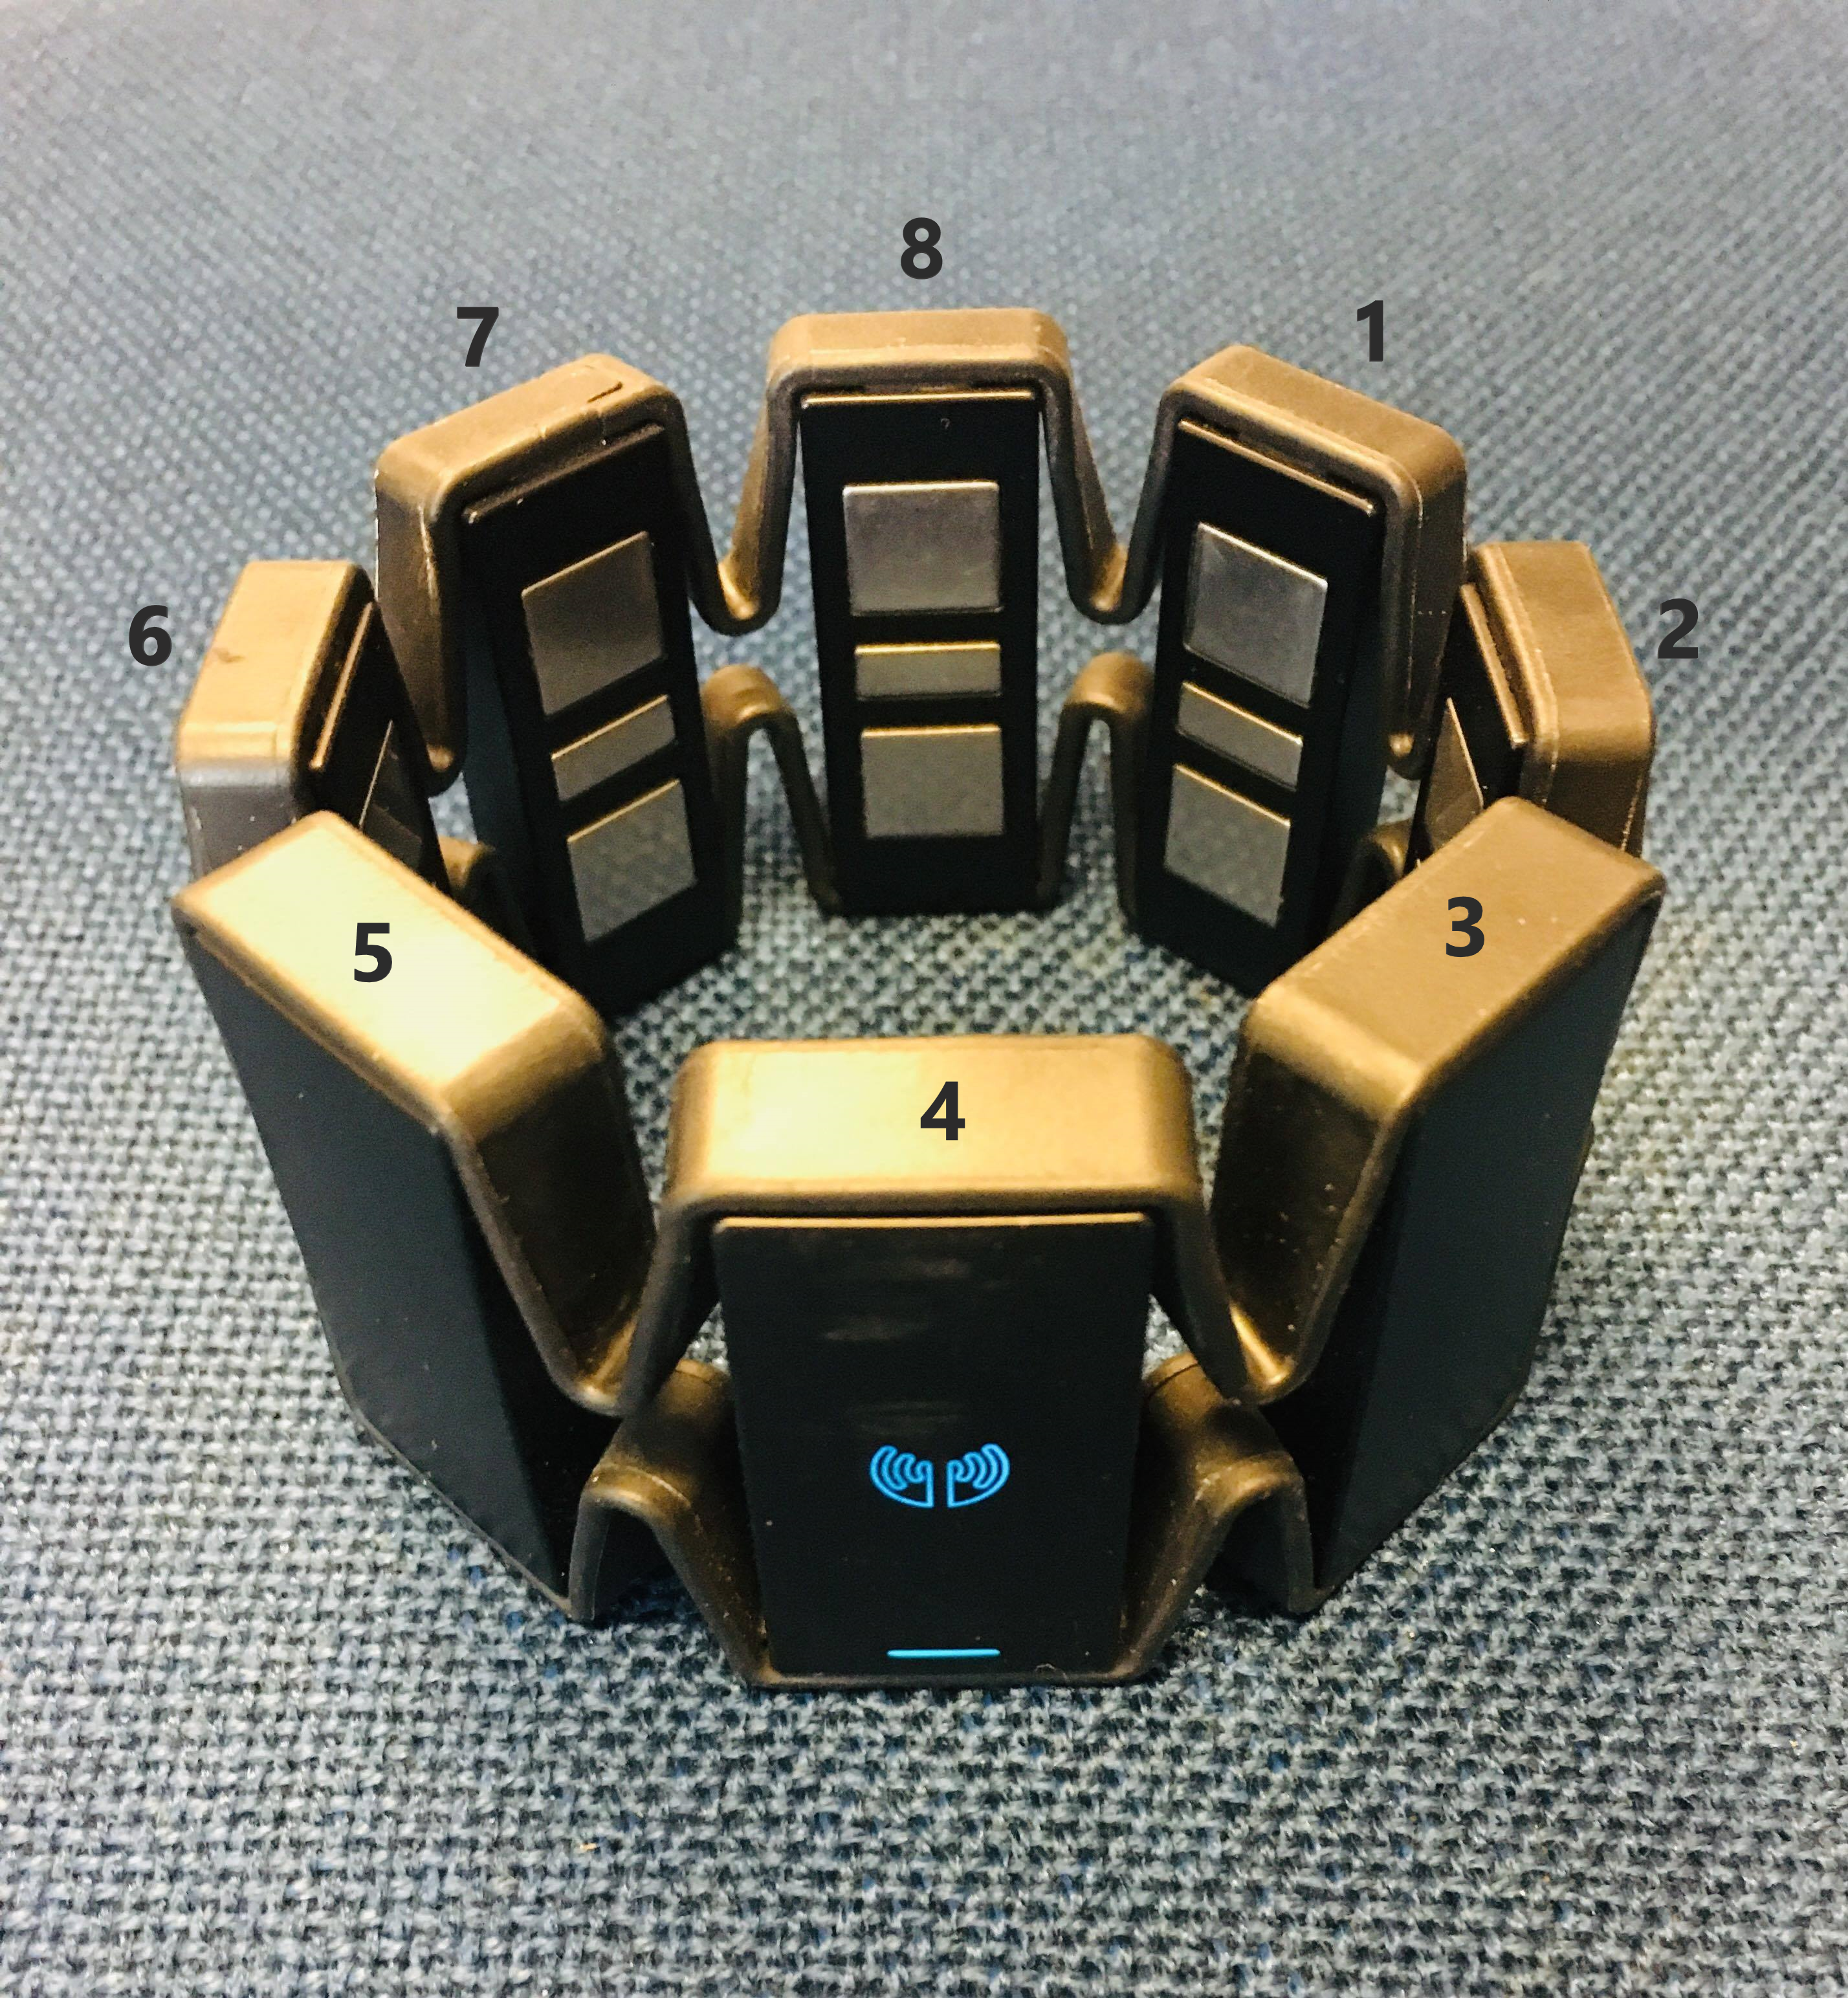
\includegraphics[width=.4\textwidth]{figures/MYB}  
	\caption{Image of the Myo armband from Thalmic Labs. Electrode channel 1 corresponds to the first output in the recording and electrode channel 2 as the second etc., as seen in \figref{fig:Emg_rot}.}
	\label{fig:MYB} 
\end{figure}
%\section{Prosthetic Control Strategies}

Throughout the development of myoelectric prosthetics, different control schemes have been derived, tested and some implemented in commercially available devices. Complexity and dexterity are dependent on the control system and before choosing a method it must be considered, which control method would be ideal for the proposed closed loop system. As presented in \secref{intro}, the feedback should provide information of the current prosthetic state. A control method which is intuitive and facilitates focus on the experienced feedback is therefore desired. 

\subsubsection{Sequential myoelectric control}


Velocity based strategies can be combined all major control schemes of switch-based, sequential and simultaneous. Switch-based is a simplistic, but slow control approach and it quickly gets impractical and non-intuitive when increasing the number of DoF's to be replaced as the intended movement is unrelated to the acquisition site \cite{Wurth2014}. Intuitiveness and naturalness in prosthetic control can be achieved through simultaneous control, where more than one DoF is controlled at a time \cite{Farina2014}. Dis ved simultan

Sequential control gives....

 Often signal from several electrodes are captured. An assumption is that given a consistent movement task is performed the muscles will exhibit a unique activation pattern, and that features extracted from each signal for each movement type can be used to distinguish between different movement types. Hence, complex EMG-signal patterns can be assigned to discrete movement classes, thus also allowing for control of several DoF's.  \cite{Farina2014,Wurth2014}  \\
This approach is more intuitive as it does not demand the need for switching between DoF's, and lowering the amount of effort the user has to put in completing a task. 

\section{Data Processing}
In order to use the acquired data most optimally in the myoelectric prosthetic control scheme the data must be processed. In this processing, undesired frequencies are filtered out and features that represents the data are extracted from segments of the data in order to obtain more information about the movement than what is only contained in the raw EMG signal. This data processing will be covered in the following sections. 

\subsection{Filtering}
To remove unwanted frequencies from the EMG signal, it should be filtered. According to the Nyquist Theorem, the rate the signal is sampled with must be at least twice the highest frequency contained in the signal to archive a non-aliased digital recording. However, as mentioned in \secref{sec:MYO}, the MYB samples with a rate lower than the highest frequency in the EMG spectrum, without having any analogue bandpass filter implemented. The rationale behind incorporating a digital anti-aliasing filter is therefore defeated. Implementing a digital high-pass filter with a corner frequency at 10 Hz to remove low frequency artefacts would, however, be desirable. \cite{Cram2012} 

\subsection{Feature Extraction}
Instead of only utilizing the raw EMG signal in a control scheme, features are extracted to exploit more representations of the EMG signal that optimally results in robust control. Various independent features can be extracted from the signal either from the time domain, frequency domain or the time-frequency domain. Most commonly features from the frequency and time domain are used. When extracting frequency domain features it is required for the EMG signal to transformed into the frequency domain. This takes more computation time compared to extracting features directly from the time domain. For this reason features in the time domain are usually favoured. \cite{Phiny2012} Especially used are the Hudgins features: Mean Absolute Value (MAV), Zero Crossings (ZC), Slope Sign Changes (SSC) and Waveform Length (WL) \cite{Hudgins1993}. However, both ZC and SSC represent the frequency content of the signal, which most likely has been distorted by the low sample rate. When using the MYB for EMG acquisition an alternative set of features has been suggested by Donovan et al. to extract from the data \cite{Donovan2017}. These features are so called space domain feature, since they exploit the relationship between the output from the electrode channels. When evaluating data acquired from the MYB the space domain features increased classification accuracy by 5 \% in a LDA-based control scheme compared to using the Hudgins features \cite{Donovan2017}. A final consideration to make when choosing features is to avoid redundancy as they then would not provide additional information about the signal. 

\subsection{Segmentation}
The extraction of features are done in discretely segmented windows of data, instead of calculating the features from instantaneous values. In online control, the length of windows is a compromise between classification accuracy and delay in prosthetic control. Often an window overlap is implemented. This is a technique applied to ensure short delays, while still enabling a high classification accuracy. When applying an overlap values from the previous window is reused in the current window. The amount of overlap chosen is significant for the performance of the control scheme.  Generally, it is recommended to have window lengths of 150-250 ms and use a 50 $\percent$ overlap. Choosing a large overlap will result in short delays, but worse classification accuracy and vice versa. When using the MYB it is important to take the low sample rate into consideration, as a window will contain less data compared to if the sampling was appropriate to the EMG frequency properties. \cite{Menon2017} Short windows will therefore likely result in worse classification accuracy compared to appropriately sampled data segmented in identical window length.
% but other studies using the MYB for data acquisition have used window lengths of 260 ms with a sliding window overlap of 235 ms \cite{Cote-Allard2017} 

\section{Classification}
For the myoelectric prosthesis to know which movement to perform, it needs to know how to differentiate between the movements it will be trained to perform. For this purpose classification is a commonly applied model. The classification model, or classifier, is given known data consisting of features extracted from the raw EMG signals, which were recorded while the user was performing different movements. If each of the known feature data sets related to each movement is known they can be labelled appropriately, and the classifier will then know which data represents which movement. Each label is known as a class and the process of labelling the data is called supervised learning. The known data is also called training data, hence this process is called training the classifier. If the classifier is trained properly, it is able to categorize unknown data accurately into the correct class. This is what happens online when using a pattern recognition-based mypelectric prosthesis. The classifier is, however, only able to categorize unknown data into one of the trained classes. \\
A frequently used supervised classifier for myoelectric prosthetic control is the Linear Discriminant Analysis (LDA). An advantage of using LDA is that it enables robust control, while having a low computational cost. LDA will be used in this project as a control scheme and an overview of the theory behind LDA will be given in the following section.

\subsection{Linear Discriminant Analysis} 


fitcdiscr(classInput,moveLabel,'DiscrimType','pseudolinear', 'ScoreTransform','none','HyperparameterOptimizationOptions','bayesopt')

pseudolinear: all classes have the same covariance matrix. The matrix is inverted by the used the pseudo inverse

none: the confidence scores are not transformed

bayesopt: uses bayes optimization to yield minimum loss in cross validation
\section{Proportional Control}
After the motor function has been determined, a mapping of the control output needs to be performed. The advantage of providing a continuous output to the actuator proportional to the contraction intensity compared to a one-speed controller is that the user has the possibility of grasping objects quickly, while still being able to perform more slow and dexterous tasks. Additionally, proportional control resembles the human neuromotor system, which makes it more intuitive. \cite{Fougner2012} 

A widely used proportional control scheme is linear regression \cite{Fougner2012}. Here, a dependent output value can be calculated based on a function of an independent input value. In the case of using several electrode channels as when using the MYB, the output needs to be computed based on several independent values. For this purpose multivariate linear regression would be appropriate:

\begin{equation}
	\hat{Y} = \alpha+\beta_{1}X_{1}+\beta_{2}X_{2}+\cdots+\beta_{i}X_{i}+\epsilon_{i}
\end{equation}

where $\hat{Y}$ is the control output and $X_{i}$ is the independent input values, where the index $i$ will correspond to the number of electrode channels in the MYB. $\alpha$ and $\beta$ are the estimated value of $\hat{Y}$ at $X$ = 0 and estimated regression coefficients, respectively. The absolute values of the recorded EMG signals can be used directly as the independents input value in such a proportional control scheme. \cite{Zar2009} However, a regression model needs to be estimated for each motor function in the control system. Then the appropriate regression model will be selected based on the classification output.  
\section{Performance Evaluation}

Evaluating the performance of a derived control system can be achieved through the completion of various tasks. If available, the system can be interfaced with a myoelectric prosthesis, and based on the completion of tasks mimicking daily life functionality (e.g. grasp and movement of objects), performance can be evaluated \cite{Mastinu2018}. Otherwise, virtual environments have been widely used showing movements of virtual prostheses \cite{Powell2014} or by moving a cursor to targets resembling motor function, where performance can be quantified through measurements based on Fitts' Law \cite{Scheme2013,Wurth2014,Hahne2014}. An obvious measure to observe is the completion rate (CR), which is the ratio of reached targets compared to the total number of targets. This describes the overall ability the user has when using the control system. Path efficiency (PE) can be used to observe how efficiently continuous movement control is achieved by comparing the distance travelled to reach a target to the most direct route. To observe how well the user can keep the system at rest and control velocity, stopping distance (SD) and overshoot (OS) can be measured. The former measures the distance travelled at times where no movement is intended, and the latter tracks the number of times the user reaches a shown target, but leaves before completion. \cite{Scheme2013}


\chapter{Study Objective}


In summary, there is still a need for myoelectric prosthetic devices to fully close the neural loop by providing amputees with proprioceptive feedback to lower the need for visual attention. As presented in \secref{SoA} most studies have focused on providing exteroceptive feedback, while only very few studies have investigated how proprioceptive information could be conveyed to aid prosthetic control in cases where visual attention is less wanted. Using the modality of electrotactile stimulation as a mean of transferring information of the prosthetic state offers multiple stimulation parameters which can be modulated through several channels enabling possibilities for intuitive and meaningful sensory feedback. However, even though several opportunities present themselves in modulating the stimulation amplitude, frequency and active channels, it would be of great interest to investigate which modulation would lead the sensory feedback to be perceived most intuitively. As stated in \secref{Maxxx} the frequency cannot be controlled individually for each pad in the electrode, thus a feedback scheme modulating frequency will not be investigated in this study. \\ 
Investigating whether spatially coded or amplitude coded information assists control the most when neglecting visual attention, will provide insight into which parameters future configurations should encapsulate. This leaves the following study objective: 

\begin{center}
	\textit{Test and evaluate two novel stimulation schemes, one based on modulating amplitude and one based on spatial localization of activation, for conveying sensory feedback of the prosthesis state in a closed-loop prosthetic control system.}  
\end{center} 


\chapter{Methods}


Applying the knowledge acquired regarding myoelectric prosthetic control and feedback stimulation, the following section will document the implementation of the two novel feedback configurations, and the remaining requirements needed to test the usability of these in a closed-loop system. The methods chapter will contain sections documenting the implementation of study design, feedback configurations, data acquisition, data processing, fitting of prosthetic control system, validation of subjects' control abilities, feedback configuration training, feedback configuration evaluation and statistical analyses.      
\section{Study Design}

In order to investigate whether amplitude or spatial based electrotactile feedback aids prosthetic control the most when removing the visual dependency, an experiment had been set up. A feedback coding scheme based on spatial activation and a feedback scheme based on amplitude modulation has been developed and will be presented later in \secref{ref til schmemes}. \\
XX subjects were recruited and randomly assigned to one of two groups. An overview of the total subject population and group demographics can be seen in \tabref{tab:demo}. Prior to enrollment, the subjects were assessed to meet the inclusion criteria stated in the experimental protocol, which can be found in \secref{Ex_protocol}. The subjects were handed the experimental protocol prior to the experiment session and gave an introduction to the background of the study and the different task the subjects would have to go through. Upon enrollment, the subjects were asked to sign an informed consent form (Fordi?). The experiment has been ethically approved by (Tilføj specifikationer).

\begin{table}[H]
	\caption{Overview of total subject population and group demographics.}\label{tab:demo}
	\begin{tabular}{llll} \hline
		& \textbf{Age, mean(std)} & \multicolumn{2}{c}{\textbf{Gender n(\%)}} \\ \cline{3-4}
		&                & Female          & Male           \\ \hline
		\begin{tabular}[c]{@{}l@{}}\textbf{Total}\\ (n = X)\end{tabular}   & \multicolumn{1}{c}{X(X)}    & X(X)       & X(X)      \\
		\begin{tabular}[c]{@{}l@{}}\textbf{Group 1}\\ (n = X)\end{tabular} & \multicolumn{1}{c}{X(X)}    & X(X)       & X(X)      \\
		\begin{tabular}[c]{@{}l@{}}\textbf{Group 2}\\ (n = X)\end{tabular}    & \multicolumn{1}{c}{X(X)}    & X(X)       & X(X)      \\ \hline
	\end{tabular}
\end{table}

The experiment was designed such that each subject was trained and tested in using both feedback schemes along with control during a one session experiment. A graphical illustration of the main stages that the subject went through can be seen in \figref{fig:std}. For all subjects data used to build the control system was acquired first. Secondly, the subjects were given time to familiarize with the control system and subsequently, the achieved control was assessed through a target reaching test. Finally, sensory thresholds used for feedback were determined for the subject. Subjects assigned to group 1 went through four steps of training and test using scheme 1 followed by the same four steps using scheme 2. The opposite was applicable for group two which started with scheme 2 followed by scheme 1. The next sections will further document the implementation and execution of the experiment.     

\begin{figure}[H]                 
	\includegraphics[width=.59\textwidth]{figures/std_design}
	\caption{Graphical illustration showing the stages of the experiment. Firstly, the stages common for all subjects followed by the group dependent stages.}
	\label{fig:std} 
\end{figure}

\section{Acquiring Control System Training Data}

As presented in \secref{patter}, for the classification scheme to differentiate between movements, it has to be trained with EMG data acquired while performing each movement. Training data was acquired using the MYB placed around the thickest part of the dominant forearm while the subject performed wrist pronation, writst supination, open hand, closed hand and rest. The subsequent section will document how the data used for training the classifier was acquired. \\
First, a baseline recording was made, where the subject was instructed in keeping the hand perfectly still. The baseline consisted of a 15 second recording and was subtracted from each of the other recordings to reduce baseline noise. If the signal was below the baseline amplitude it was set to zero. \\
During a muscle contraction two main states can be recognized: a transient state, described by inconsistent myoelectric activity as the muscle length is changed, and steady state, where a constant firing rate is reached. \cite{Mobarak2014} Classification is often based solely on steady state data, however, including transient state might make for a more robust classifier as the delay until steady state is reached is eliminated \cite{Boschmann2013,Mobarak2014a}. \\
%

\begin{figure}[H]                 
	\includegraphics[width=1\textwidth]{figures/trapezoid}  
	\caption{The trapezoidal plot (left) and contraction validation plot (right) used during acquisition of the training data. The trapezoidal plot represented the contraction amplitude requested and the black cursor represented the currently elicited contraction intensity. }
	\label{fig:GUI} 
\end{figure}
\vspace{-1em}

To feed the classifier with training data representing muscle contractions with varying force, different fractions of maximum contraction force were recorded. In the process of obtaining training data for each movement, the same four contraction were carried out: a prolonged maximum voluntary contraction (pMVC) recording and 40 $\percent$, 50 $\percent$ and 70 $\percent$ of the pMVC recordings.
The pMVC was recorded for 15 seconds where the subject was instructed to elicit the contraction with a maximum contraction force which could be held steady without fatigue, over the course of the 15 seconds. This resulted in an pMVC for each channel in the MYB, which was calculated as the mean of the absolute values of the EMG signal for each channel. The mean for each channel was used as a maximum reference when acquiring the subsequent fraction recordings. \\
Acquisition of the 40 $\percent$, 50 $\percent$ and 70 $\percent$ fraction of pMVC were done using a graphical user interface (GUI) made in MATLAB 2018b, which can be seen in \figref{fig:GUI}. The image shows the trapezoidal trajectory the subject were instructed to follow using the black cursor, where the height of the cursor was calculated as the mean absolute intensity across all channels of the elicited muscle contraction. The cursor would automatically move positively along the x-axis in relation to time. The high plateau of the trapezoid represented either the 40 $\percent$, 50 $\percent$ or 70 $\percent$ fractions of the pMVC. Data were recorded during 2.5 seconds rest periods in the beginning and end, a 2.5 incline transition, 5 second steady state and 2.5 second decline transition, summing to a total time of 15 seconds. However, only data recorded during the steady state and the last and first second of the incline and decline of the transition phase, respectively, were used to train the classifier. \\
The additional plot, seen on the right in \figref{fig:GUI}, plotted the amplitude of each of the eight channels in the MYB and were used by the investigators to assess whether the performed movements were done correctly. If the amplitude of the channels responsible for the performed movement shifted rapidly, or if channels not responsible for the performed movement were active, it would indicate that the subject did not perform a pure contraction and the recording would have to be redone.   
   
   

\section{Data Processing}
The following sections will cover which filtering, segmentation and feature extraction solutions that were decided to implement, based on the background information presented in \secref{sec:BG:dataProcessing}. 

\subsection{Filtering}
Due to the EMG-bandwidth being 10-500 Hz and taking the MYB specifications into consideration the only interest was to remove low-frequency artefact noise. Hence, a $2^{nd}$ order Butterworth high-pass filter with a cut-off at 10 Hz was implemented. The order of the filter was chosen, as fast update time was highly desired in the online prosthetic control, and a higher order might have slowed the update due to a longer computation time. The choice of implementing a Butterworth filter was due to the desire of avoiding phase shift inside the EMG bandwidth, as this could distort the fidelity of some of the extracted features. 

\subsection{Segmentation}
In online myoelectric prosthetic control, quick update time is important to maintain naturalness in the prosthesis motion, while still ensuring robust classification. A windowing of 200 ms with 50 \% overlap was therefore chosen. This would update the prosthesis motion state every 100 ms and segment 40 samples per window to feed the classifier. In initial tests, this proved adequate to yield smooth and reliable prosthesis motions, when using the MYB for EMG acquisition. 

\subsection{Feature Extraction}
For this project it was decided to extract the space domain features recommended by Donovan et al. \cite{Donovan2017}, due to the increased classification accuracy obtained compared to using Hudgins features when applying the MYB for data acquisition. The features formulated in \cite{Donovan2017} were MAV, Mean MAV (MMAV), Scaled MAV (SMAV), Correlation Coefficient (CC), Mean Absolute Difference Normalized (MADN), MAD Raw (MADR) and Scaled MADR (SMADR). Additionally, it was decided to extract the Hudgins feature, WL, to exploit frequency related information of the signal in the classification. All these features will be explained in the following text. \\
MAV is a commonly used feature to represent information on muscle contraction intensity and how much force a subject needs to produce to perform a movement at a given intensity. Its changes are linearly proportional with contraction intensity; the more intense the contraction is the higher the feature value will be and vice versa. For one window in the $i^{th}$ channel, MAV is calculated as:

\begin{equation} \label{eq:MAV}
MAV_i=\frac{\sum\limits_{n=1}^{ws}|x_i[n]|}{ws}
\end{equation}

where $x_i[n]$ denotes the $n^{th}$ raw sample from channel $i$ and $ws$ denotes window size or number of samples in one window. \\
Scaling MAV with the mean of MAV across all channels will remove the dependency of specific movement intensity - some movements produce higher mean intensities than others at the same fraction of the MVC. The average of MAV across all channels is denoted MMAV and is calculated as: 

\begin{equation} \label{eq:MMAV}
MMAV=\frac{\sum\limits_{i=1}^{8}MAV_i}{8}
\end{equation}

MAV scaled by MMAV is denoted SMAV and is calculated as follows for each window in the $i^{th}$ channel:

\begin{equation} \label{eq:SMAV}
SMAV_i=\frac{MAV_i}{MMAV}
\end{equation}

Each EMG channel in the MYB records a mixture of sources. Some individual sources can affect multiple channels, which will increase the correlation between channels, while other more local sources might only affect a single channel, which decreases the correlation. To represent the correlation between channel $i$ and the neighbouring channel $i+1$, Donovan et al. proposed the calculation of a correlation coefficient (CC), which is expressed as: 

\begin{equation} \label{eq:CC}
CC_i=\frac{\sum\limits_{n=1}^{ws}X_i[n]X_{i+1}[n]}{ws}
\end{equation}

where $X_i[n]$ is the $n^{th}$ sample from channel $i$ in one window after the sample has been normalized. The normalization is done by subtracting the mean of raw samples from each samples followed by dividing the resulting values with their standard deviation.  \\
In an effort to further represent the relationship between channels, the mean of the absolute value of the difference between normalized channel values was calculated. This is referred to as mean absolute difference normalized (MADN), and is expressed as:

\begin{equation} \label{eq:MADN}
MADN_i=\frac{\sum\limits_{n=1}^{ws}|X_i[n]-X_{i+1}[n]|}{ws}
\end{equation}

To decrease the computational denseness of first calculating the normalized values as done with CC and MADN, MAD was calculated using just the raw samples. This is referred to as MADR and is expressed as:

\begin{equation} \label{eq:MADR}
MADR_i=\frac{\sum\limits_{n=1}^{ws}|x_i[n]-x_{i+1}[n]|}{ws}
\end{equation}

Similar to MAV, MAD is affected by movement intensity and is therefore scaled by MMAV, which results in the final space domain feature SMADR: 

\begin{equation} \label{eq:SMADR}
SMADR_i=\frac{MADR_i}{MMAV}
\end{equation}

Finally, to increase the amount information the classifier based its decisions upon, the Hudgins feature WL was included. WL represents both amplitude and frequency content of the signal by measuring the summed absolute difference between neighbouring samples in the signal in channel $i$ in one window: 

\begin{equation} \label{eq:WL}
WL_i=\sum\limits_{n=1}^{ws-1}|x_{i}[n+1]-x_i[n]|
\end{equation}

To avoid redundancy in signal representation only SMAV, CC, MADN SMADR and WL were used to train the classifier and for online control. 


\section{The Virtual Closed-Loop Prosthesis} \label{sec:vp}

In order to test the usability of the two sensory feedback configurations in a closed-loop control system, a prosthesis which accommodated this was simulated. As no commercial or research prostheses were available in this project, a virtual system resembling prosthetic control was made. Using a virtual prosthesis also had the benefit of providing no sounds that might indicate the prosthetic state during evaluation tests.

The aim was to develop a system which could provide control and feedback of two degrees of freedom. In \figref{fig:meth:gridmap} is a depiction of a grid system and a black cursor symbolizing the different possible prosthetic states and the current prosthetic state, respectively, where each square corresponded to a prosthetic state. Performing supination would make the cursor move to the right into one of two possible states, while performing pronation would make the cursor move left into one of two states. Performing the closed hand movement would make the cursor move downwards into one of four possible states and performing open hand would make the cursor move upwards. In total, the prosthesis could achieve a total of 25 different states, which represented single DoF movements or combinations of two DoFs. However, as the control was sequential it was only possible to move the cursor in a single DoF at a time along an axis. In each of the squares, a unique electrotactile feedback was provided in each of the two feedback configurations, as explained in \secref{sec:feed}, thus ascribing four states for each DoF.      
     

\begin{figure}[H]                 
	\includegraphics[width=0.9\textwidth]{figures/gridmap2}  
	\caption{Image of the grid map and cursor used in the experiment. Performing supination moved the cursor to the right, pronation moved it to the left and closing the hand moved it downwards. For left handed subjects the rotational movements were reversed. Opening the hand moved the cursor upwards, and was used as a correction movement if needed.}
	\label{fig:meth:gridmap} 
\end{figure}
%hand movements used 

%The Grid 

\section{The Prosthetic Control System}

Having extracted features from the three EMG datasets of one movement for each of the four movements, the control system could be build in order to achieve online recognition of movements. The implementation of the control system was divided into two parts. To achieve recognition of performed movement a classifier was trained, however, this only produces a recognition of a movement and does not reflect the intensity of which the movement is being performed with. Therefore, following the recognition of the performed movements a linear regression model was implemented to achieve proportional control. 

\subsection{Movement Classification}

Online classification of movements was accomplished by implementing a LDA classifier. As presented in \secref{patter} the classifier needed to be trained using data from each movement. Hence, the five features extracted for each of the 40 $\percent$, 50 $\percent$ and 70 $\percent$ fraction of the pMVC for one movement were assembled into one labeled matrix. The same was done for the three remaining movements. A fifth class was labeled rest and its matrix only contained the features from a single rest acquisition. These matrices were made for the data acquired from each of the eight channels in the MYB. All matrices were assembled into one training matrix with labels for each movement. Using the \textit{fitcdicsr}-function in MATLAB a LDA classifier was trained by feeding it the training matrix. Hereby, the classifier was trained in separating 5 classes using linear decision boundaries. During online use, the \textit{predict}-function was used to evaluate features from new input data in the classifier and decide which movement there was being performed.    


\subsection{Proportional control}  
When a movement was decided upon by the classifier, the proportional control provided the control system with an actual output to move the virtual prosthesis. For this purpose a multiple linear regression model was created for each of the four movements, through the MATLAB function \textit{fitlm}. The models were fitted with the MAV features extracted from the fraction of pMVC data as well as the mean of the pMVC data. The data was scaled such that the pMVC data was set to 1 and the remaining data was scaled in relation to that. In the online control, the output of the decided regression models was written such that it would move in the direction described in \secref{sec:vp}. The output from the regression models was limited to a maximum of 1, meaning that maximum level of activation detecting was the pMVC level. This was equivalent to moving the cursor 1 cm on the computer screen. Thus, the cursor had a maximum speed of 1 cm per output. As the grid system was quadratic with 20 cm in length, each DoF had a full actuation speed of 2 seconds at maximum activation. Another threshold implemented was a minimum activation of at least 15 $\percent$ for a movement to count, otherwise no output would be provided. This idea behind this implementation was to provide a more stable resting state in addition to the classifier. 


\section{Online Control Training and Test} \label{sec:meth:contraintest}

After the acquisition of data training data and the training of the classifier, two stages where the subject could familiarize themselves with the control and test how well they were able to use the control system, were implemented. It was highly critical that the subject was able to achieve sufficient control abilities such that it would not be due to poor control that a subject was not able to perform well when combined with sensory feedback in the final evaluation tests. However, as the classifier only had five classes, representing five separable movements to distinguish between, a robust online control was achieved in an evaluation test during pilot tests after short training trials. Therefore, the need for subject training could be kept to a minimum.  

\subsection{Familiarization with Control} \label{sec:meth:contrain}

At first, the subject was presented with an image of the grid, which can be seen in \figref{fig:meth:gridmap}, in \secref{sec:vp}. The subject was able to control a cursor and navigate around inside the grid by performing supination to go right, pronation to go left, open and closed hand to go up and down, and rest to stand still. The familiarization was separated into two stages. In the first stage, the user had three minutes to get acquainted the functionality of the control moving the cursor shown in \figref{fig:C1} (a). The cursor acted as a direct output of the control. During the three minute familiarization, the subject was instructed in training unflawed performance of each movement and the transition from a movement to rest. In the second stage, the visual feedback in the form of the cursor was made more discrete. This was done by making the cursor invisible and instead highlighting the outlines of the target that contained the cursor. This discretized cursor representation was included to make the visual feedback identical in resolution to the sensory feedback. The discrete visual feedback can be seen in \figref{fig:C1} (b). Again the subject had three minutes to familiarize with the control. 

\begin{figure}[H]
	\subfigure[Illustration of the cursor used during the first familiarization stage.]
	{\includegraphics[width=0.34\textwidth]{figures/cursor}}
	\hspace{0.9cm}
	\subfigure[Illustration of the cursor used during the second familiarization stage. ]
	{\includegraphics[width=0.34\textwidth]{figures/blue}}
	\caption{Illustration of the cursor used in the two stage familiarization with control.  Using this cursor in (a) the subject was informed the exact location of cursor in a square. Using this cursor in (b) the subject was provided with the information of which square the cursor was in, but not the exact location of the cursor inside the square. }
	\label{fig:C1}
\end{figure}

\subsection{Evaluation Test} \label{sec:meth:contest}

After completion of the two stages of familiarization, a target reaching test was carried out. In this project, performance evaluation will be carried out in a virtual environment through a Fitts' Law based target reaching test. In this test, a square was highlighted with red and the subject would have to move the discretized cursor to the desired target and dwell inside it for 1.5 seconds in order for it to be deemed reached. The subject had 30 seconds to reach a target. The test was designed such that each of the 24 squares in the grid was to be reached. When a target was either reached or the time to reach the target ran out, the cursor would be reset to the neutral position (first row, third column in \figref{fig:meth:gridmap}). \\
The target reaching test was made such that a measure of how well the subjects was able to use the control system could be obtained. Hereby it also acted as a reference for the later comparisons with control in combination with the two feedback schemes. Furthermore, if the investigators deemed the achieved subject control insufficient, the investigators could choose to exclude the subject. From the target reaching test, performance measures of completion rate, time to reach a target and length travelled to reach a target were extracted for performance evaluation.



\section{Determination of Stimulation Levels}

Having completed the prosthetic control part of the experiment, the next step was to determine the subject's sensory threshold levels, which would be used to convey feedback information.

In order to provide meaningful tactile feedback to the subject, a range of distinguishable sensory threshold levels had to be determined for the subject. As presented in \secref{sec:vp} the virtual prosthesis had a range of one to four active motion states and one passive state. Hence, four thresholds based on amplitude values were determined to accommodate four levels of feedback in the amplitude scheme. Furthermore, since the sensory sensitivity varies across different locations of the circumference of the arm, the sensory threshold levels had to be determined for each individual pad in the electrode array. Sensory threshold levels were found by slowly increasing the amplitude while fixating the pulse width and frequency at 500 $\mu$s and 50 Hz, respectively. 

In the first round, the lowest level was determined, which will be referred to as the perception threshold. For each pad, the amplitude was set to start at 0 $\mu $A and then increase in steps of 100 $\mu$A per second. The subject was instructed in reporting when electrical stimulation could be sensed and that the subject was sure the activated pad was the origin of the perceived stimulation. The pad was deactivated and reactivated once more with the determined amplitude value for a second verification. This process was carried out for each pad starting from pad 1 to 16. Subsequently, the subject was presented with the determined amplitude values in each pad, such that the sensation in the current pad was compared to the neighboring pad. This was carried out such that the determined amplitude values could be readjusted to achieve more homogeneous sensation intensities across all pads.  

In the second round, the fourth level thresholds, referred to as tolerance threshold, were determined using the same procedure as in round one. The tolerance threshold was defined as the highest amplitude the subject felt pleasant. The starting amplitude was in this round, however, the perception threshold. The amplitude was set to increase in steps of 200 $\mu$A per second. The amplitude was increased until the subject reported that the threshold was reached, the stimulation was causing functional muscle activation or a maximum of 10000 $\mu$A was reached. Again the amplitude values were readjusted to achieve homogeneous sensation intensities. Throughout the process of determining sensory threshold levels, the subject was facing away from the computer screen to avoid bias from observing the visual increase of amplitude values.  

Intermediate threshold levels 2 \textit{lvl2} and 3 \textit{lvl3} were calculated for the $i^{th}$ pad based on the perception \textit{p} and tolerance \textit{t} threshold levels as: 

\begin{equation}
lvl2_i = p_i + \frac{1}{3} \cdot (t_i - p_i)
\end{equation}

\begin{equation}
lvl3_i = t_i - \frac{1}{3} \cdot (t_i - p_i)
\end{equation}

       
\section{Feedback Configurations} \label{sec:feed}

The fundamental interest of this project was to develop two novel, intuitive and useful feedback schemes to convey proprioceptive information through electrotactile stimulation and evaluate which one would aid control the most. The following section will present the two developed spatial and amplitude feedback schemes. All anatomical directions are explained with the hand being pronated as reference.      

\subsection{Spatial Configuration}

The spatial feedback scheme was created with the interest of achieving an intuitive way to convey the feedback by focusing stimulation to localized regions on the skin. An illustration of the spatial feedback scheme can be seen in \figref{fig:spatial}. The idea behind this configuration was to communicate rotation movements by rotating the activated electrode pads and to convey the closed hand movement by narrowing distance between active electrodes. \\
The intent was to break down the number electrode pads into two groups: one upper and one lower. The upper eight pads (5-12) were used to convey information of the rotational DoF using four pads for either side.  The four pads were divided into pairs of two, where the first from the center in e.g. pronation would be activated when the cursor entered the first level in the grid system. Likewise, the second level pair would be activated when the cursor entered the second level. Hence, during a transition from neutral to level one and level one to level two, the subject should feel the stimulation moving either laterally or medially depending on the position of the cursor. Finally, this meant that when the virtual prosthesis was in a supinated state the stimulation should be felt in the anterior lateral region of the arm, while when the virtual prosthesis was is in a pronated state stimulation should be felt in the anterior medial region of the arm.   \\
The lower eight pads (1-4 and 13-16) were used to convey information about the closed hand DoF. The pads were paired in an opposite manner for each of the four levels respectively, e.i. 4 and 13, 3 and 14, 2 and 15 and 1 and 16. As the hand would move to one closed hand state out of four possible, a certain pad pair would activate. Transiting from neural to fully closed, the subject should feed the stimulation converging on the posterior side of the arm. The virtual prosthesis was able to be in states, which was a combination of the two DoFs. In these cases the feedback would be a combination of any upper and lower pair, resulting in the activation of four pads simultaneously. In the spatial feedback scheme, it was chosen to use the second amplitude level determined to enhance the subject's perception of the stimuli. 

\begin{figure}[H]                 
	\includegraphics[width=0.55\textwidth]{figures/El_array_spatial}  
	\caption{Illustration of the developed spatial scheme, which is based on different pads being activated depending on the level of the state the cursor is located in. The level assigned to the various electrode pairs corresponded to levels of prosthesis state in \figref{fig:meth:gridmap}. The highest number of possibly activated pads was four at a time.}
	\label{fig:spatial} 
\end{figure}


\subsection{Amplitude Configuration}

Compared to the spatial configuration where the feedback was given through dynamically changing the pads activated, the amplitude configuration instead conveyed feedback in three greater regions and solely modulated the amplitude of the stimulation. The upper eight pads were again used for the rotational DoF, illustrated in \figref{fig:amplitude}. Pads 5-8 were activated at pronated states using threshold levels 2 and 3 for states 1 and 2, respectively. The same was applicable for supinated states using pads 9-12. \\
For conveying information about closed hand pads (1,2,15,16) were used. In these, threshold levels 1-4 were used for states 1-4, respectively. When in a grid position corresponding to a combined DoF prosthetic state, eight electrodes would be active in amplitude levels relative to the grid position. It was chosen to use groups of four electrode pads to exploit the largest number of pads in the electrode array, while still maintaining a symmetric distribution of possible active pads. \\ 
In this scheme, attention to the recognition of stimulation localization should be less. Instead, the subject would have to focus on discriminating between the intensity of stimulation in the regions which were active.           

\begin{figure}[H]                 
	\includegraphics[width=0.55\textwidth]{figures/El_array_amplitude}  
	\caption{Illustration of the developed amplitude scheme. Here, the amplitude of the active pads would increase with the increase of the prosthetic state; the higher the level the higher the current amplitude of the given electrodes. The level of amplitude strength assigned to the various electrodes corresponded to levels of prosthesis state in \figref{fig:meth:gridmap}. The highest number of possibly activated pads was eight at a time.}
	\label{fig:amplitude} 
\end{figure}








\section{Feedback Training}
After determining the amplitude thresholds, the subject was trained in understanding the sensory feedback. Depending on which group the subject was allocated to, the subject was either trained in understanding the spatial or amplitude scheme first. The structure of the training was, however, the same. The feedback training was divided into two phases: familiarization and reinforced learning. These phases will be presented in the following sections.

\subsection{Familiarization} \label{sec:meth:FBtrainingFam}
In the familiarization phase, the subject was presented with the sensation of 12 different grid squares and 12 grid squares indirectly, while observing which grid location corresponded to which sensation. This was carried out by the investigators by moving the cursor seen in \figref{fig:gridmap_FBfam} with the arrow keys on the keyboard. One press with an arrow key would move the cursor in a different grid square in the direction relative to the arrow key pressed. Pressing return would place the cursor in the staring point (the third grid square in the first row). The order of which grid square the cursor would be moved to can be seen in \figref{fig:gridmap_FBfam}. After reaching a designated square, the cursor would be reset to the starting point. When moving the cursor to a grid square not adjacent to the staring point, the feedback from the transition grid squares would be felt. This transition is transferable to practical proportional prosthetic control/feedback, where the transition from rest to an outer prosthetic position is apparent. When moving the cursor to the grid squares 9, 10, 11 and 12, representing combined DoF positions, the direct route (moving fully in one direction and then the other) was used. In the familiarization phase, the cursor would be moved fully horizontally and then vertically. This enabled stimulations relative to all grid square to be included in the familiarization, without setting all grid squares to be designated targets. This design was chosen due to the single DoF direction being assessed to be most important to get familiar with, and to save time while still exposing the subject to all possible stimulations. Time spend in designated squares was approximately four seconds and time spend in transition squares was approximately two seconds.

\begin{figure}[H]                 
	\includegraphics[width=0.55\textwidth]{figures/gridmap_FBfam}  
	\caption{Illustration of the order the cursor would be moved to which grid squares in. The numbered grey squares are designated squares. After reaching a designated square, the cursor would be reset to staring position (the grid square the cursor is located in).}
	\label{fig:gridmap_FBfam} 
\end{figure}

\subsection{Reinforced Learning} \label{sec:meth:FBtrainingRe}
The reinforced learning phase consisted of two blocks, in which all grid squares were designated squares. When a designated square was reached the investigator asked the subject about the location of the cursor. If the subject answered incorrectly, the investigator would reveal the actual location of the cursor. The stimulation related to the designated would be active until the subject answered. Afterwards, the cursor would be reset to the starting point. \\
The difference between the two blocks was the order and path to the designated squares, which was predetermined by the investigators. The blocks were, however, identical for all subjects. The path to a designated square was the direct route. However, which direction that would be moved in first was predetermined by the investigators. Thus, the transition stimulations would be felt by the subject before the designated was reached. This design was implemented to avoid bias in being accustomed to always receiving stimulation related to the same DoF first before the other. Time spend in transition squares was approx. two seconds. 
\section{Combining Control and Sensory Feedback}
After the subject was trained in understanding one of the feedback schemes, the sensory feedback was combined with prosthetic control. Similar to the control step of the study, see \subref{sec:meth:contraintest}, the subject would go through a familiarization phase before undergoing evaluation tests. These stages will be explained in the following sections.

\subsection{Familiarization}
This stage was similar to the second stage control training, see \secref{sec:meth:contrain}, with the addition of receiving sensory feedback. The subject was instructed in refreshing the prosthetic control, while adapting further to the feedback related to the various prosthesis states as well the transitions felt when changing prosthesis state. These focus point was assessed most beneficial to train in order to perform well in the final evaluation test. 

\subsection{Final Evaluation Test}
This evaluation test was similar to the evaluation test from the control step, see \secref{sec:meth:contest}, with the addition of receiving sensory feedback. In this test, the prosthesis state would, however, not be visualized. Thus, the subject had to use the sensory feedback to determine the prosthesis state and reach the highlighted targets. The target reaching test was performed two times consecutively. Again the completion rate, time to reach a target and length travelled to reach a target were extracted for performance evaluation.
\section{Statistics}
Due to the low sample size, comparisons was made using non-parametric statistics. Wilcoxon signed rank test was applied as comparisons was made on related samples obtained from a two block study design. A significance level of 5 $\percent$ was used.

\chapter{Results}
	
\urlstyle{same}
\printbibliography
\clearpage



\cleardoublepage
% BILAG
\begin{appendices}
\chapter{Appendices}
\section{Experiment Protocol}

\textbf{Project Title} \\
Evaluation of electrotactile feedback schemes in combination with myoelectric prosthetic control - closing the loop. 

\textbf{Information on Investigators} \\
The investigators are biomedical engineering Master students at Aalborg University. 

\textbf{Background} \\
Losing an upper limb can be hugely debilitating and can result in lowered quality of life due to restrictions in function, appearance and sensation. As a mean to regain the loss, transradial amputees can receive a functional prosthesis, where the majority are controlled by muscles signals, or electromyography (EMG). However, still 25\% of EMG prosthesis users reject their device, where a major reason for the low satisfaction is due to lack of sensory feedback.
Many advancements have been made in the academic community to improve function accuracy. However, combining function with sensory feedback, thus closing the motor/sensory loop, is still a scarcely investigated area. Therefore, this experiment will combine the control of a prosthesis with sensory feedback delivered via electrotactile stimulation electrodes placed on the forearm. During the experiment the subjects will test two different feedback configurations while controlling a virtual prosthesis, represented as a cursor on a computer screen.  

\textbf{Purpose} \\
The purpose of the experiment is to compare how subjects' perform in an evaluation test when receiving feedback from two different electrotactile stimulation configurations, respectively, in a closed loop virtual prosthesis. This might provide information on which feedback that seems more intuitive to use in practice in a prosthesis.


\textbf{Research Aim} \\
Test and evaluate two novel stimulation schemes, one based on modulating amplitude and one based on spatial localization of activation, for conveying sensory feedback of the prosthesis state in a closed loop prosthetic control system.

\textbf{Experiment Duration} \\
To be estimated.

\textbf{Inclusion Criteria} \\
The subject must be:
\begin{itemize}
	\item able bodied or transradially amputated as the highest degree of upper limb amputation.
	\item at least 18 years of age.
	\item able to understand, read and speak English and/or Danish.
	\item assessed by the investigators to comply with the instructions given during the experiment.
\end{itemize}

\textbf{Exclusion Criteria} \\
The subject must:
\begin{itemize}
	\item not have any diseases/conditions that may influence sensory perception.
	\item be willing to receive low amplitude current stimulation. 
\end{itemize}

\textbf{{\Large Experiment Procedure}} \\
\newline
The main focus of the experiment is for the subject to be able correctly interpret the two sensory feedback schemes. The grid illustrated in \figref{fig:gridmap} is the map the subject will be able to move around inside. Each square in the map will deliver a different stimulus corresponding to the motion state of the virtual prosthesis, represented as the black cursor. The square with center in the origin (square with cursor inside in \figref{fig:gridmap}) corresponds to resting state and will provide no sensory feedback. The remaining squares in the first row will deliver stimuli corresponding to only the wrist rotation degree of freedom (DOF), and the remaining squares in the third column will deliver stimuli corresponding to the closed hand DOF. The remaining squares will deliver a stimulation based on a combination of the two DOFs. The further away from resting state a square is, corresponds to a higher muscle contraction level.
The images located at each axis represent the hand movements needed to be performed to move the cursor in a desired direction. The control system will only react on one movement performed at a time. Thus, the cursor is only able to move along one axis at a time and not diagonally.

\begin{figure}[H]                 
	\includegraphics[width=0.78\textwidth]{figures/gridmap}  
	\caption{Image of the grid map and cursor used during all trainings and tests.}
	\label{fig:gridmap} 
\end{figure}

Before the final evaluation test is carried out the subject will be trained in controlling the cursor, trained in interpreting the sensory feedback and trained in interpreting the sensory feedback while controlling the cursor. The following order represent the chronology of the tasks the subject needs to undergo:

\begin{enumerate}
	\item Record EMG signals needed to build the prosthetic control system.
	\item Train the subjects ability to control the cursor via letting the subject move freely around inside the grid map.
	\item Perform target reaching test to evaluate the subject's ability to control the cursor.
	\item Record current amplitude thresholds needed to build the sensory feedback schemes.
	\item Train the subject's ability to interpret the single DOF sensory feedback of feedback scheme 1 by exposing the subject three times to each of the eight stimuli squares.
	\item Perform reinforcement learning on the eight squares from step 5 two times with sensory feedback from scheme 1.
	\item Perform validation test on the eight squares from step 5 two times with sensory feedback from scheme 1.
	\item Train the subject's ability to control the cursor while receiving sensory feedback from scheme 1 via letting the subject move freely around inside the grid map.
	\item Perform target reaching test where the cursor is invisible to evaluate how well the subject is to utilize the sensory feedback from scheme 1 regarding the cursor location.
	\item Redo step 5-9 with sensory feedback from scheme 2.
\end{enumerate}


\textbf{{\Large Hand Movements Used in the Experiment}} \\

\begin{figure}[H]                 
	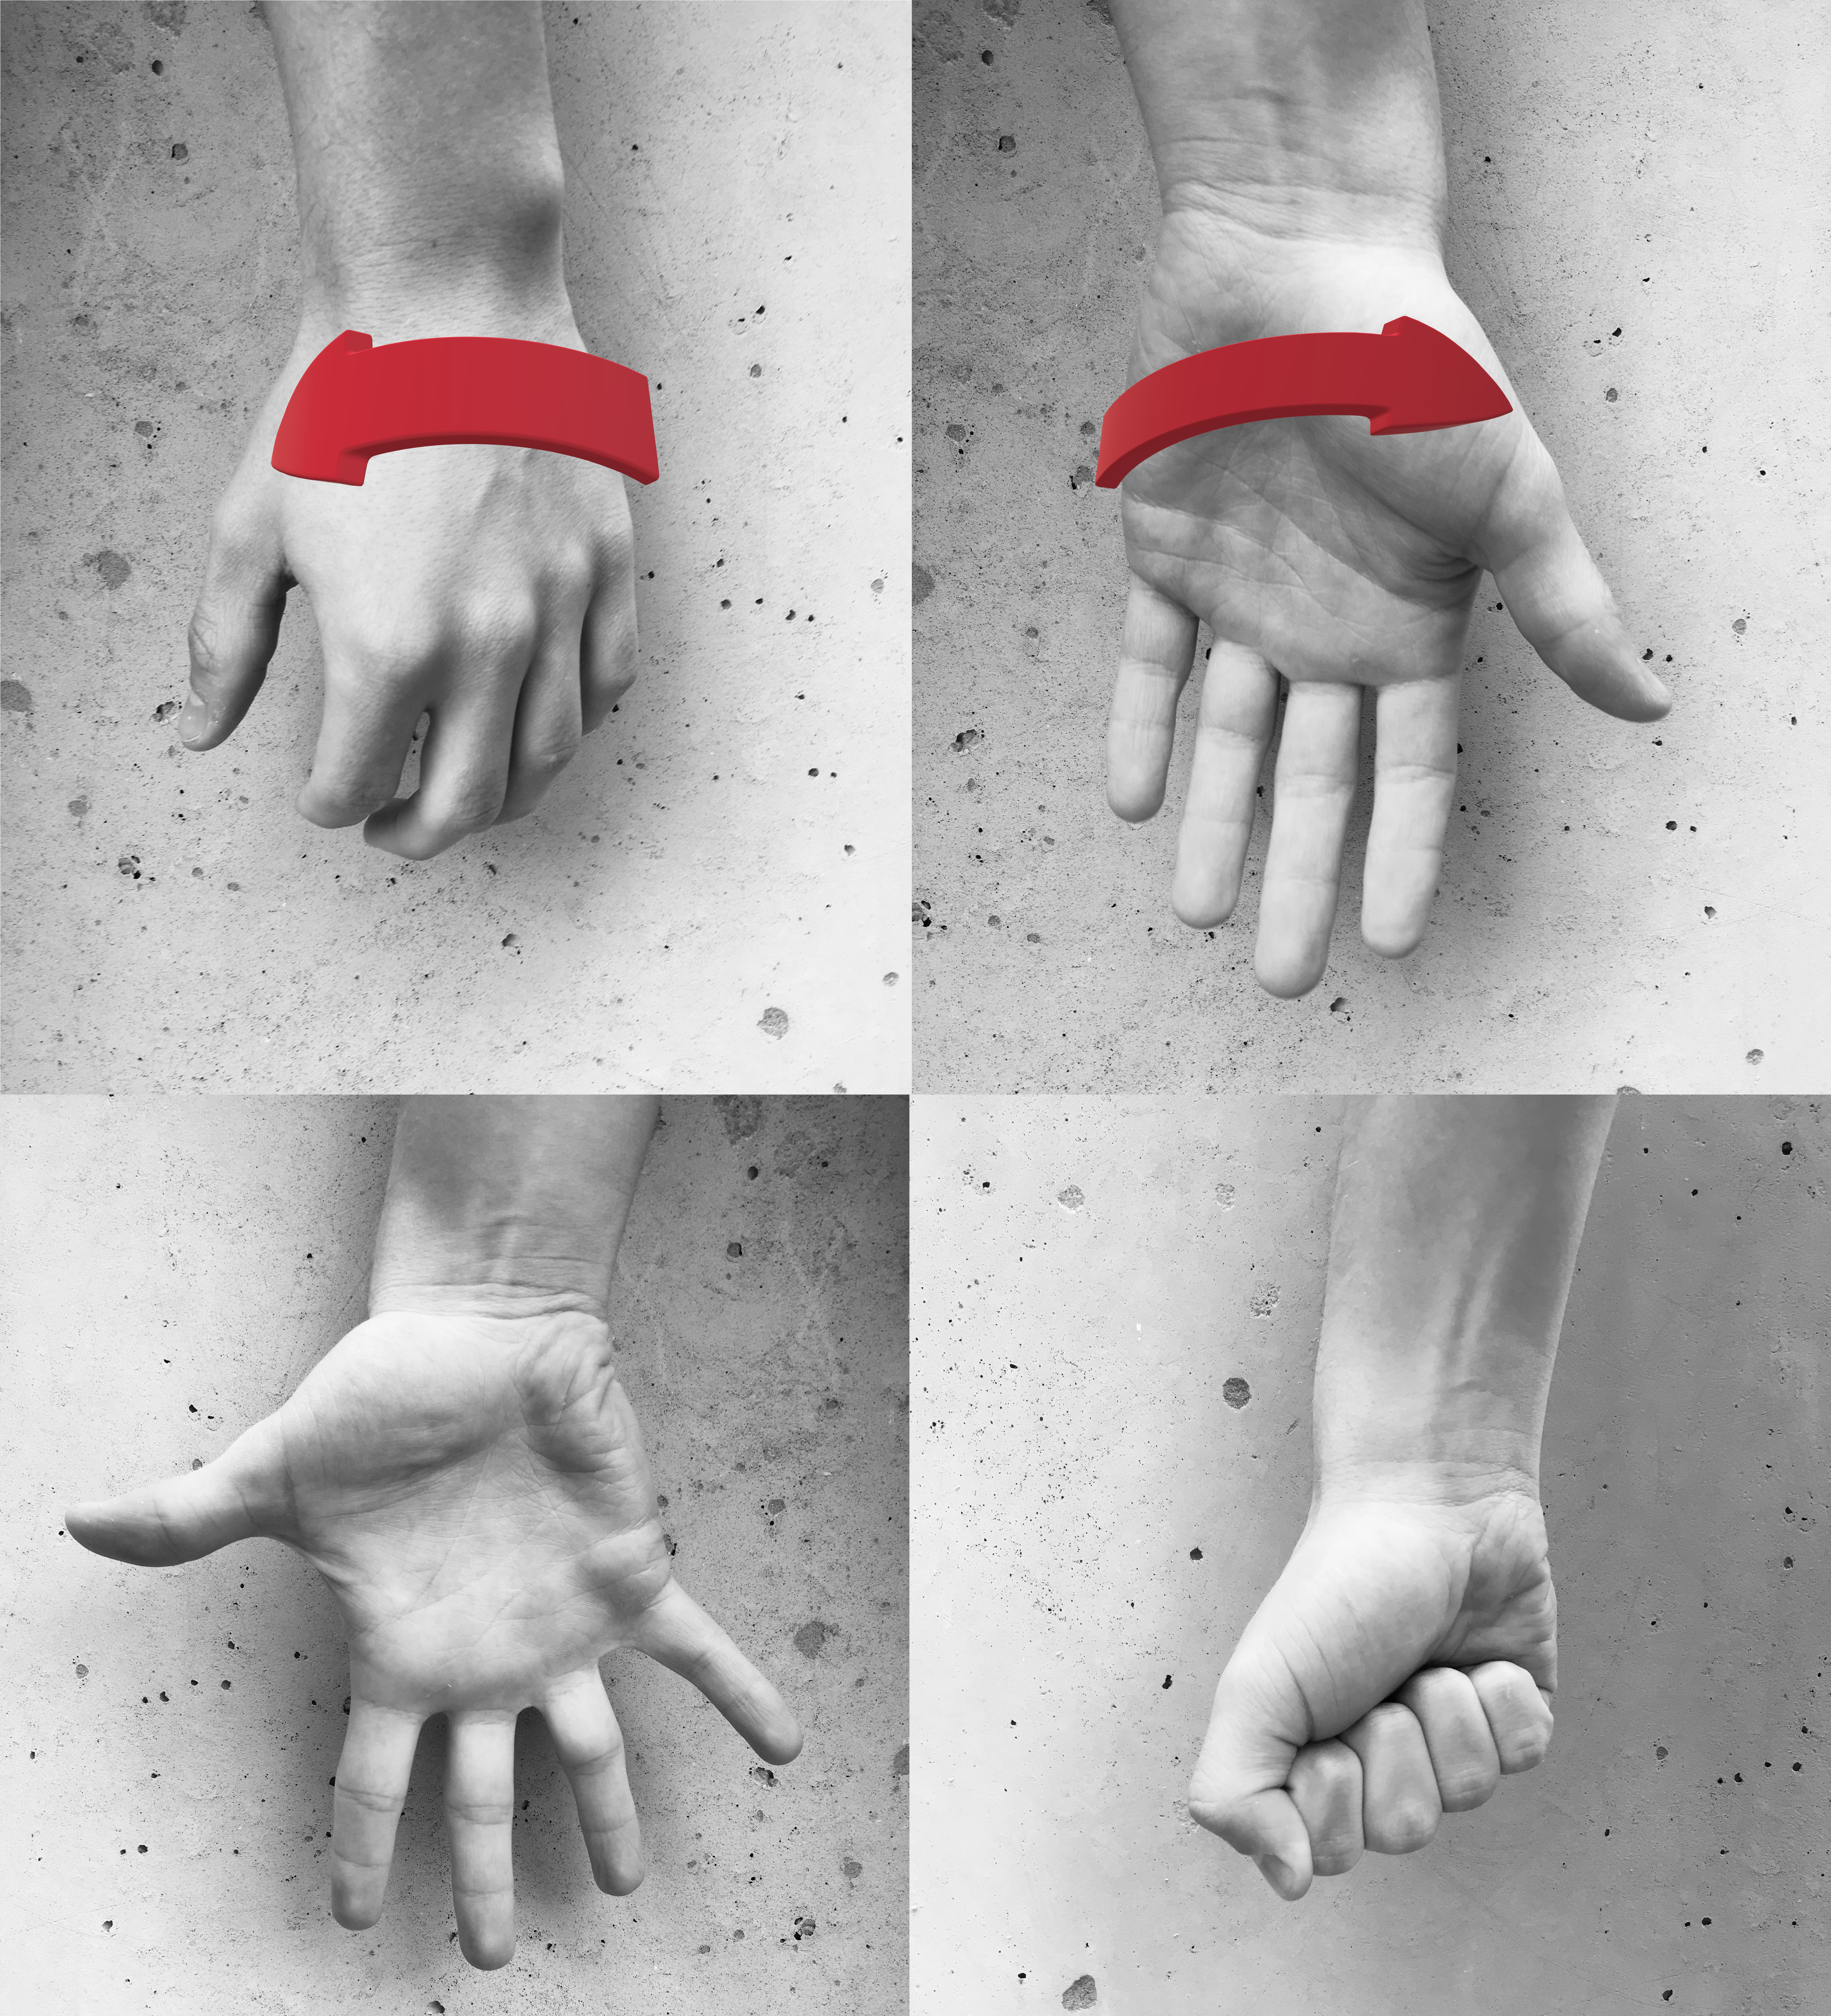
\includegraphics[width=0.78\textwidth]{figures/handmovements}  
	\caption{Image of the hand movements used in the experiment. From top left corner: Wrist pronation, wrist supination, opened hand and closed hand.}
	\label{fig:handmovements} 
\end{figure}

\textbf{{\Large Experiment Setup}}


%\newpage
\section{Experiment Introduction Letter}

\textbf{Project Title} \\
Evaluation of electrotactile feedback schemes in combination with myoelectric prosthetic control - closing the loop. 

\textbf{Experiment Purpose} \\
When a person gets amputated on the lower arm, he/she can receive a functional prosthesis. This is controlled by muscle signals from the user, where the muscle signals are translated into a prosthesis movement. However, many functional prostheses do not provide sensory feedback, which results in some users to abandon their prosthesis. \\
The purpose of the experiment is to compare how subjects perform in an evaluation test when receiving feedback from two different electrical stimulation configurations, while controlling a virtual prosthesis. The results might provide information on which feedback that seems more intuitive to use in a real prosthesis.   

\textbf{Experiment Overview} \\
The experiment will take place in the laboratory $D3-107$ at Aalborg University. The duration of the experiment is estimated to be 2 hours and 30 minutes. During the experiment a myoelectric armband will be placed on the dominant forearm and will be used to record muscle activity during the performance of four different hand gestures. Subsequently, a test of the ability to reproduce the gestures will be made. \\
Afterwards, an electrode armband, capable of delivering electrical stimulation at 16 different locations will be placed on the non-dominant arm. A test to determine the electrical perception and tolerance level for the subject will then be carried out. The subject will then be made familiar and trained in understanding two different feedback configurations representing possible states which the virtual prosthesis might produce. A test of the subjects ability understand the feedback while making the trained hand gestures will be made right after familiarization and training for each feedback configuration. \\
On the day of the experiment please refrain from using any types of sensory deprivation drugs (painkillers and the likes). The test subject will not receive monetary reimbursement upon completing the experiment.  
\end{appendices}


\end{document}
